\documentclass[border=4pt]{standalone}
\usepackage{tikz,amsmath}
\usetikzlibrary{arrows.meta,patterns}
\definecolor{nuit}{HTML}{190F3C}\definecolor{bleu}{HTML}{3746FF}
\definecolor{corail}{HTML}{FF808B}\definecolor{corailf}{HTML}{D6455A}
\definecolor{bleuclair}{HTML}{9BA3FF}
\newcommand{\vv}[1]{\underline{#1}}
\begin{document}
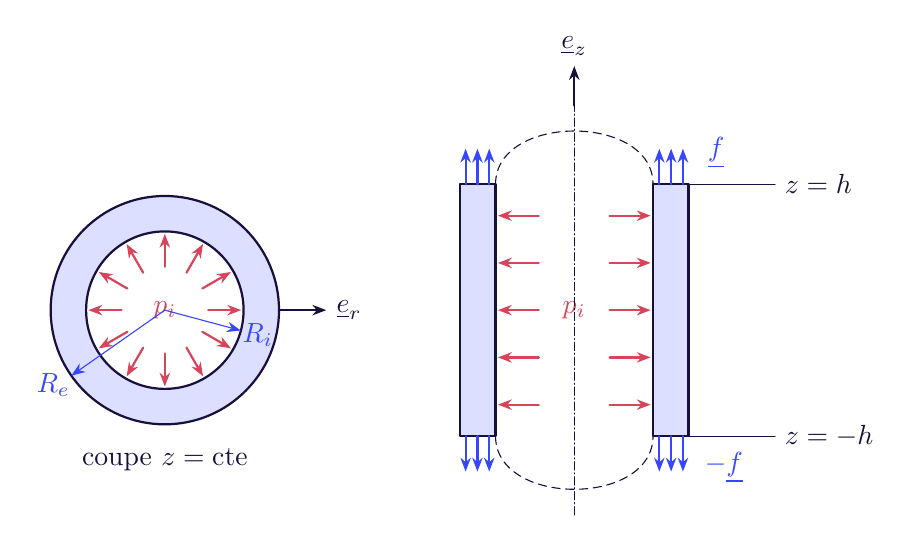
\begin{tikzpicture}[line cap=round,line join=round,>={Stealth[length=5pt]},
  every node/.style={text=nuit}]
  \def\Ri{1.0}\def\Re{1.45}
  % ---------- Coupe transversale ----------
  \fill[bleuclair!35,even odd rule] (0,0) circle (\Re) (0,0) circle (\Ri);
  \draw[nuit,thick] (0,0) circle (\Re) (0,0) circle (\Ri);
  \foreach \t in {0,30,...,330}{
    \draw[->,corailf,thick] ({0.55*\Ri*cos(\t)},{0.55*\Ri*sin(\t)}) -- ({0.97*\Ri*cos(\t)},{0.97*\Ri*sin(\t)});}
  \node[text=corailf] at (0,0) {$p_i$};
  \draw[->,bleu] (0,0) -- ({\Ri*cos(-15)},{\Ri*sin(-15)});
  \node[text=bleu] at ({1.22*cos(-15)},{1.22*sin(-15)}) {$R_i$};
  \draw[->,bleu] (0,0) -- ({\Re*cos(215)},{\Re*sin(215)});
  \node[text=bleu] at ({1.15*\Re*cos(215)-0.05},{1.15*\Re*sin(215)}) {$R_e$};
  \draw[->,nuit,thick] (\Re,0) -- (\Re+0.6,0) node[right] {$\vv{e}_r$};
  \node at (0,-\Re-0.45) {coupe $z = \text{cte}$};
  % ---------- Coupe longitudinale ----------
  \begin{scope}[xshift=5.2cm]
    \def\h{1.6}
    % fonds (en pointillés : ils ne font pas partie du domaine étudié)
    \draw[nuit,densely dashed] (-\Ri,\h) .. controls (-\Ri,\h+0.9) and (\Ri,\h+0.9) .. (\Ri,\h);
    \draw[nuit,densely dashed] (-\Ri,-\h) .. controls (-\Ri,-\h-0.9) and (\Ri,-\h-0.9) .. (\Ri,-\h);
    % parois
    \foreach \s in {-1,1}{
      \fill[bleuclair!35] (\s*\Ri,-\h) rectangle (\s*\Re,\h);
      \draw[nuit,thick] (\s*\Ri,-\h) rectangle (\s*\Re,\h);}
    % pression intérieure
    \foreach \z in {-1.2,-0.6,...,1.3}{
      \draw[->,corailf,thick] (-0.45,\z) -- (-0.97*\Ri,\z);
      \draw[->,corailf,thick] (0.45,\z) -- (0.97*\Ri,\z);}
    \node[text=corailf] at (0,0) {$p_i$};
    % effort axial transmis par les fonds
    \foreach \s in {-1,1}{
      \foreach \x in {1.08,1.23,1.38}{
        \draw[->,bleu,thick] (\s*\x,\h) -- (\s*\x,\h+0.45);
        \draw[->,bleu,thick] (\s*\x,-\h) -- (\s*\x,-\h-0.45);}}
    \node[text=bleu] at (\Re+0.35,\h+0.4) {$\vv{f}$};
    \node[text=bleu] at (\Re+0.45,-\h-0.4) {$-\vv{f}$};
    % axe et cotes
    \draw[nuit,densely dash dot] (0,-\h-1.0) -- (0,\h+1.0);
    \draw[->,nuit,thick] (0,\h+1.0) -- (0,\h+1.5) node[above] {$\vv{e}_z$};
    \draw[nuit] (\Re,\h) -- (\Re+1.1,\h) node[right] {$z = h$};
    \draw[nuit] (\Re,-\h) -- (\Re+1.1,-\h) node[right] {$z = -h$};
  \end{scope}
\end{tikzpicture}
\end{document}
